% =====================================================================
%  Conpot ICS/SCADA Honeypot — project presentation (LaTeX Beamer)
% ---------------------------------------------------------------------
%  Compile:  tectonic presentation.tex
%            or latexmk -pdf presentation.tex   (pdflatex, run twice)
%            or upload this folder to https://overleaf.com and press Compile
%  Figures live in ./figures/ (charts generated from the real conpot.log).
%  TODO: put the student's name + course on the title slide (marked below).
% =====================================================================
\documentclass[aspectratio=169,11pt]{beamer}

% ---- minimal base theme, fully customised below ----
\usetheme{default}
\usecolortheme{default}
\setbeamertemplate{navigation symbols}{}
\setbeamertemplate{frametitle continuation}{}

% ---- clean sans-serif fonts (helvet for text; math stays Computer Modern) ----
\usepackage[T1]{fontenc}
\usepackage{helvet}
\renewcommand{\familydefault}{\sfdefault}

\usepackage{graphicx}
\usepackage{booktabs}
\usepackage{xcolor}
\usepackage{tikz}
\usetikzlibrary{arrows.meta,positioning}
\graphicspath{{figures/}}

% ---- palette ----
\definecolor{ink}{HTML}{15303A}      % deep teal-slate — titles, bars
\definecolor{hpcyan}{HTML}{0E7490}   % accent
\definecolor{hpred}{HTML}{C0392B}    % high / tamper
\definecolor{hpgreen}{HTML}{1E8449}
\definecolor{hppanel}{HTML}{EDF2F4}  % light panel fill
\definecolor{hpmuted}{HTML}{5A6A75}  % muted grey-teal

\setbeamercolor{normal text}{fg=ink!92!black}
\setbeamercolor{structure}{fg=hpcyan}
\setbeamercolor{frametitle}{fg=ink}
\setbeamercolor{title}{fg=ink}
\setbeamercolor{block title}{fg=white,bg=ink}
\setbeamercolor{block body}{fg=ink!90!black,bg=hppanel}
\setbeamercolor{section in toc}{fg=ink}
\setbeamercolor{footline}{fg=hpmuted}

\setbeamerfont{frametitle}{series=\bfseries,size=\large}
\setbeamerfont{title}{series=\bfseries,size=\LARGE}
\setbeamerfont{block title}{series=\bfseries,size=\small}
\setbeamerfont{footline}{size=\scriptsize}

% ---- frametitle: bold title + thin accent rule ----
\setbeamertemplate{frametitle}{%
  \vspace*{0.8em}%
  {\usebeamerfont{frametitle}\usebeamercolor[fg]{frametitle}\insertframetitle}\par
  \vspace*{0.18em}%
  {\color{hpcyan}\rule{\linewidth}{1pt}}%
  \vspace*{-0.3em}%
}

% ---- bullets ----
\setbeamertemplate{itemize item}{\small\color{hpcyan}\raisebox{0.1ex}{$\blacktriangleright$}}
\setbeamertemplate{itemize subitem}{\footnotesize\color{hpcyan}\textbf{--}}

% ---- flat blocks ----
\setbeamertemplate{blocks}[rounded][shadow=false]

% ---- minimal footline ----
\setbeamertemplate{footline}{%
  \hbox{\begin{beamercolorbox}[wd=\paperwidth,ht=2.6ex,dp=1.4ex,leftskip=1.1em,rightskip=1.1em]{footline}%
    \usebeamerfont{footline}\insertshorttitle\hfill\insertsectionhead\hfill\insertframenumber\,/\,\inserttotalframenumber%
  \end{beamercolorbox}}%
}

% ---- custom title page ----
\setbeamertemplate{title page}{%
  \vfill
  {\color{hpcyan}\rule{\linewidth}{2.2pt}}\\[0.6em]
  {\usebeamerfont{title}\usebeamercolor[fg]{title}\inserttitle\par}
  \vspace{0.5em}
  {\color{hpmuted}\small\insertsubtitle\par}
  \vspace{1.3em}
  {\color{hpcyan}\rule{3.2cm}{1pt}}\\[0.8em]
  {\usebeamerfont{author}\insertauthor\par}
  \vspace{0.2em}
  {\color{hpmuted}\footnotesize\insertinstitute\par}
  \vspace{0.5em}
  {\color{hpmuted}\scriptsize\insertdate\par}
  \vfill
}

% ---- section divider frames ----
\AtBeginSection[]{%
  \begin{frame}[plain]
    \vfill
    \hspace{1.4em}{\color{hpcyan}\rule{1.2pt}{2.4em}}\hspace{1em}%
    \begin{minipage}{0.8\linewidth}
      {\color{hpmuted}\footnotesize\textbf{\MakeUppercase{Part \thesection}}}\\[0.25em]
      {\color{ink}\LARGE\textbf{\insertsectionhead}}
    \end{minipage}
    \vfill
  \end{frame}
}

\newcommand{\high}{\textcolor{hpred}{\textbf{High}}}
\newcommand{\seq}{scan $\to$ read $\to$ write}

% ---------------------------------------------------------------------
\title[Conpot ICS Honeypot]{Building and Attacking an ICS/SCADA Honeypot}
\subtitle{A Conpot decoy PLC over Modbus, SNMP, S7comm, FTP and BACnet --- live attack probes, automated log analysis and a real-time dashboard}

% TODO: replace the bracketed course/university on the title slide
\author{Khan Imaad Ali \textnormal{(22410104)}\\[3pt] Makrand Gaikwad \textnormal{(22410110)}}
\institute{[Course / Module --- University]}
\date{\today}

\begin{document}

% ===================== TITLE =====================
\begin{frame}[plain]
  \titlepage
\end{frame}

% ===================== OUTLINE =====================
\begin{frame}{Outline}
  \tableofcontents
\end{frame}

% =====================================================================
\section{Background}
% =====================================================================
\begin{frame}{Why an ICS/SCADA honeypot?}
  \begin{itemize}
    \item Industrial Control Systems (ICS/SCADA) run power, water and factory plants
          using legacy protocols --- \textbf{Modbus}, \textbf{S7comm}, \textbf{SNMP} ---
          built with \emph{little or no authentication}.
    \item These devices are increasingly reachable from the network, and attackers
          actively scan for them (Shodan, automated ICS worms).
    \item A \textbf{honeypot} is a decoy device: it looks like a real PLC, has no real
          process behind it, and \emph{logs everything an attacker does}.
  \end{itemize}
  \vfill
  \begin{block}{Goal}
    Stand up a realistic ICS honeypot, attack it over \textbf{five protocols}, and turn the
    raw honeypot log into structured events, risk scores and a live dashboard.
  \end{block}
\end{frame}

\begin{frame}{Conpot --- the honeypot engine}
  \begin{columns}[T]
    \begin{column}{0.58\textwidth}
      \begin{itemize}
        \item Open-source, low-interaction ICS honeypot from the \textbf{Honeynet Project}.
        \item Emulates a \textbf{Siemens SIMATIC S7-200} PLC.
        \item Speaks \textbf{Modbus/TCP}, \textbf{S7comm}, \textbf{SNMP}, \textbf{HTTP} ---
              plus \textbf{FTP}, \textbf{BACnet} and more --- in one container.
        \item Answers with a believable device identity, so a scanner thinks it found a
              real PLC --- then records every interaction.
      \end{itemize}
    \end{column}
    \begin{column}{0.42\textwidth}
      \begin{block}{Two halves of the system}
        \textbf{Attacker side} --- deploy Conpot, probe it, capture \texttt{conpot.log}.\\[4pt]
        \textbf{Analysis side} --- parse the log, detect attack patterns, score risk, build a
        dashboard.
      \end{block}
    \end{column}
  \end{columns}
\end{frame}

% =====================================================================
\section{Architecture}
% =====================================================================
\begin{frame}{System architecture}
  \begin{center}
  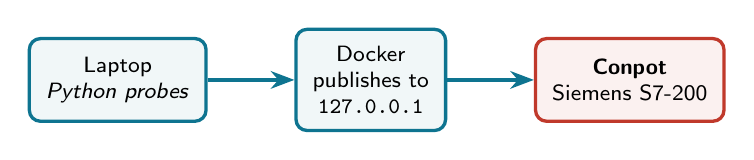
\begin{tikzpicture}[
      box/.style={draw=hpcyan,very thick,rounded corners,align=center,
                  fill=hpcyan!6,minimum height=1.05cm,font=\footnotesize,inner sep=6pt},
      arr/.style={-{Stealth[length=3mm]},very thick,hpcyan}]
    \node[box] (lap)    {Laptop\\\textit{Python probes}};
    \node[box,right=1.1cm of lap] (dkr) {Docker\\publishes to\\\texttt{127.0.0.1}};
    \node[box,right=1.1cm of dkr,fill=hpred!7,draw=hpred] (cp) {\textbf{Conpot}\\Siemens S7-200};
    \draw[arr] (lap) -- (dkr);
    \draw[arr] (dkr) -- (cp);
  \end{tikzpicture}
  \end{center}
  \vfill
  \begin{columns}[T]
    \begin{column}{0.46\textwidth}
      The Conpot \textbf{Docker} container (built from the project's custom image)
      publishes its ICS ports on \texttt{127.0.0.1}, so every probe targets localhost and
      reaches the container directly --- no separate machine needed.
    \end{column}
    \begin{column}{0.54\textwidth}
      \centering\small
      \begin{tabular}{@{}lcc@{}}
        \toprule
        \textbf{Service} & \textbf{Laptop port} & \textbf{Conpot port}\\
        \midrule
        Modbus      & 502       & 5020  \\
        S7comm      & 102       & 10201 \\
        SNMP (udp)  & 161       & 16100 \\
        HTTP        & 8080      & 8800  \\
        FTP         & 2121      & 2121  \\
        BACnet (udp)& 47808     & 47808 \\
        \bottomrule
      \end{tabular}
    \end{column}
  \end{columns}
\end{frame}

% =====================================================================
\section{Attacking the honeypot}
% =====================================================================
\begin{frame}{Attack methodology --- five probes}
  Five Python probes run from the laptop against \texttt{127.0.0.1}, each generating clean,
  labelled traffic --- the classic \textbf{\seq} chain.
  \vfill
  \begin{itemize}
    \item \textbf{Modbus} \scriptsize(pymodbus)\normalsize\ --- read coils, discrete inputs and
          registers, then \textbf{write} a holding register (value 1234), \emph{accepted} by the
          custom template: a live tamper.
    \item \textbf{SNMP} \scriptsize(pysnmp)\normalsize\ --- \texttt{GET} system OIDs and \texttt{WALK}
          the system subtree; returns the Siemens identity.
    \item \textbf{S7comm} \scriptsize(snap7)\normalsize\ --- establish an S7 session and request CPU
          identification (SZL) --- what PLC-scanning tools do first.
    \item \textbf{FTP} \scriptsize(ftplib)\normalsize\ --- anonymous control session
          (\texttt{SYST}/\texttt{PWD}/\texttt{STAT}/\texttt{HELP}).
    \item \textbf{BACnet} \scriptsize(socket)\normalsize\ --- a broadcast \texttt{Who-Is}, the
          building-automation reconnaissance move.
  \end{itemize}
  \vfill
  {\footnotesize The write + multi-protocol scan is deliberate: it is a real attacker moving from
  \emph{reconnaissance} to \emph{tampering}.}
\end{frame}

% =====================================================================
\section{Results}
% =====================================================================
\begin{frame}{What the honeypot captured}
  \begin{columns}[c]
    \begin{column}{0.54\textwidth}
      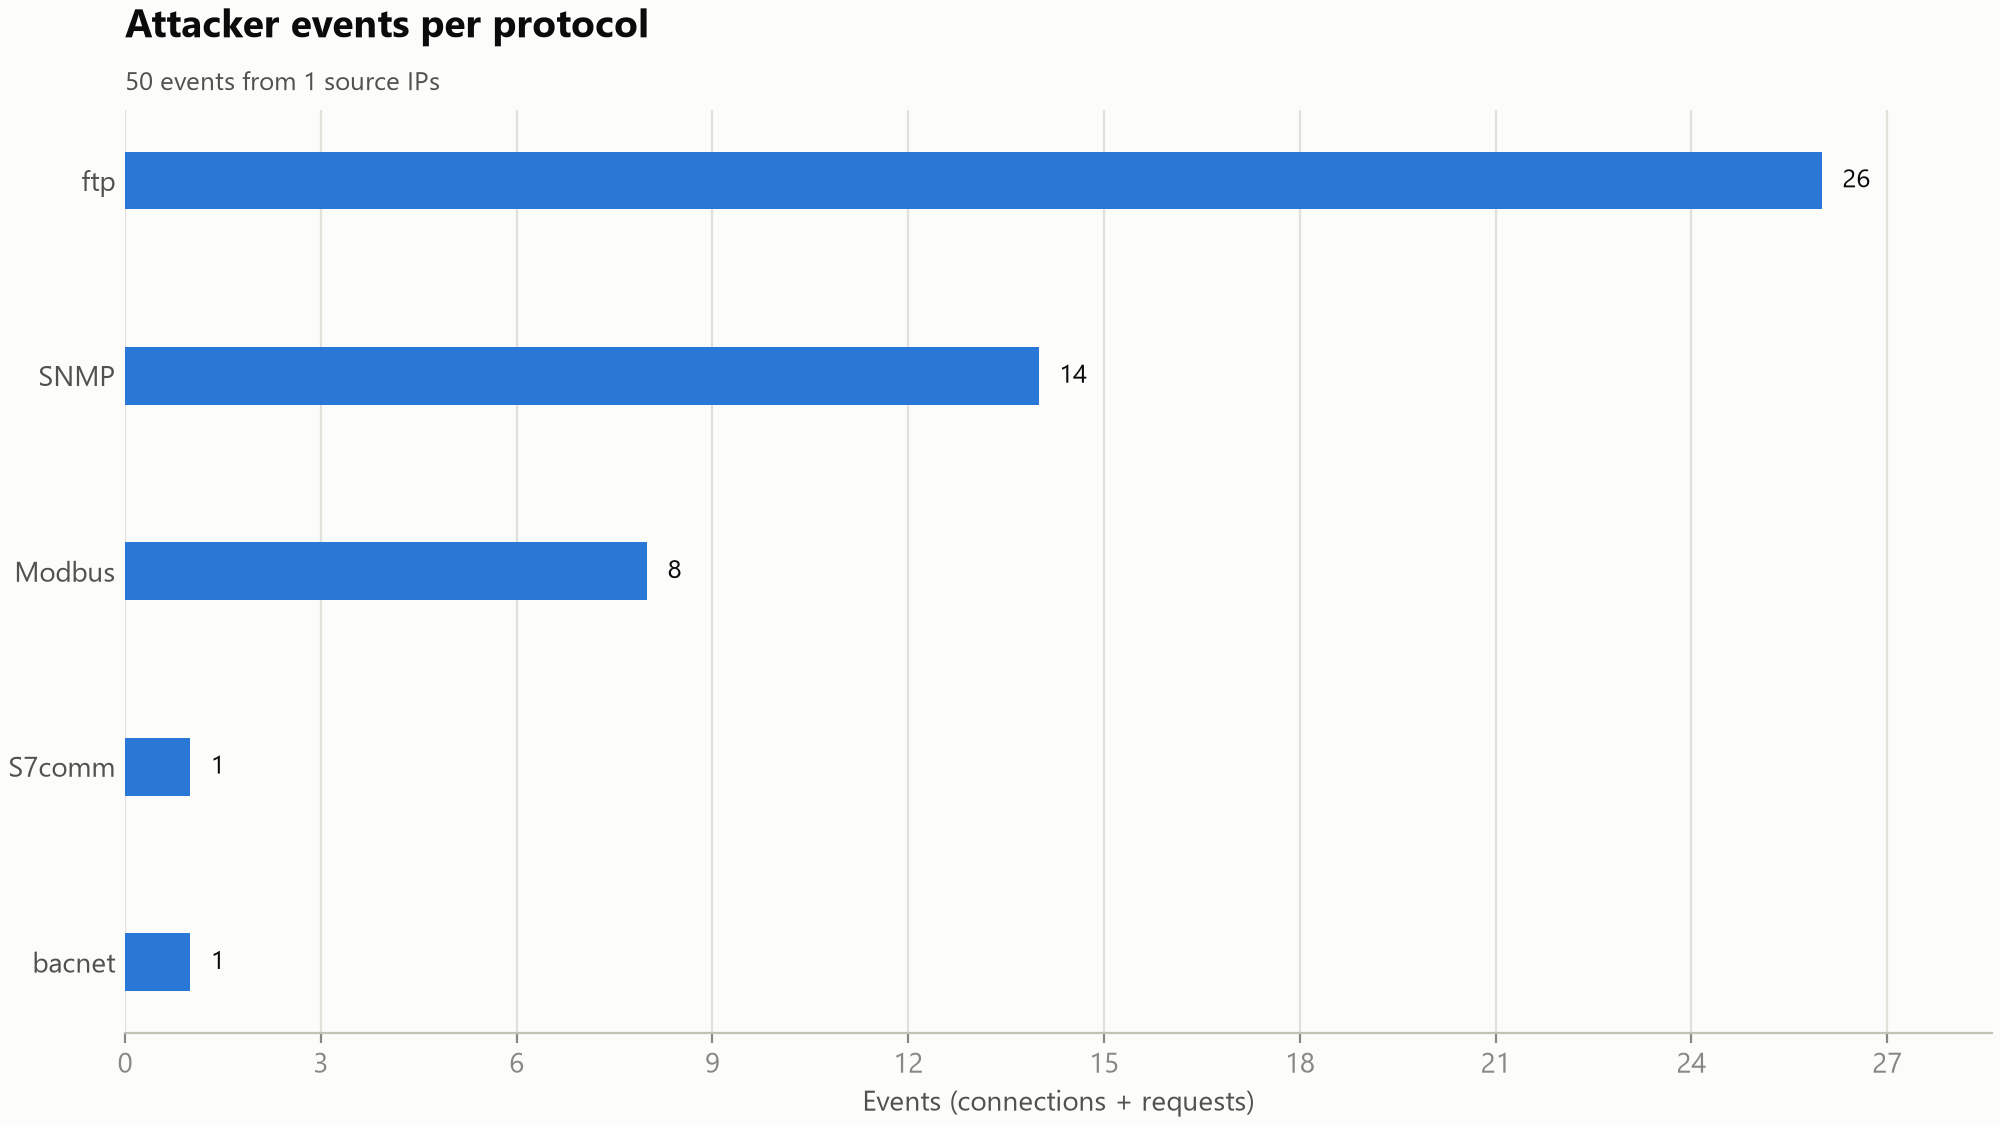
\includegraphics[width=\linewidth]{attacks-per-protocol}
    \end{column}
    \begin{column}{0.46\textwidth}
      \begin{itemize}
        \item \textbf{50 attacker events} from a single source (\texttt{172.17.0.1}, the Docker
              gateway --- i.e.\ our laptop).
        \item \textbf{FTP} (26) --- the control-session commands.
        \item \textbf{SNMP} (14) --- the full system-tree walk.
        \item \textbf{Modbus} (8) --- register reads and an accepted write.
        \item \textbf{S7comm} (1), \textbf{BACnet} (1) --- reconnaissance contacts.
      \end{itemize}
    \end{column}
  \end{columns}
\end{frame}

\begin{frame}{The deception works --- twice}
  \begin{columns}[T]
    \begin{column}{0.5\textwidth}
      \begin{block}{SNMP: a convincing identity}
        \small
        \begin{tabular}{@{}ll@{}}
          sysDescr    & Siemens, SIMATIC, S7-200 \\
          sysName     & CP 443-1 EX40 \\
          sysContact  & Siemens AG \\
          sysLocation & Venus \\
        \end{tabular}
      \end{block}
      {\footnotesize A scanner now believes this is a real Siemens PLC.}
    \end{column}
    \begin{column}{0.5\textwidth}
      \begin{block}{Modbus: real data \& a live tamper}
        \small
        Custom template --- slave 1 answers with realistic process data:\\[3pt]
        holding registers = \texttt{[1480, 1465, 85, \dots]} (pump setpoints)\\[2pt]
        input registers = \texttt{[412, 538, 1260, \dots]} (sensors)\\[4pt]
        A write of \textbf{1234} to holding register 0 is \textcolor{hpred}{\textbf{accepted}}
        --- read-back = 1234.
      \end{block}
      {\footnotesize An attacker can change the PLC's ``process'' --- the core ICS threat.}
    \end{column}
  \end{columns}
\end{frame}

% =====================================================================
\section{Log analysis \& detection}
% =====================================================================
\begin{frame}{From raw log to structured events}
  \begin{columns}[c]
    \begin{column}{0.52\textwidth}
      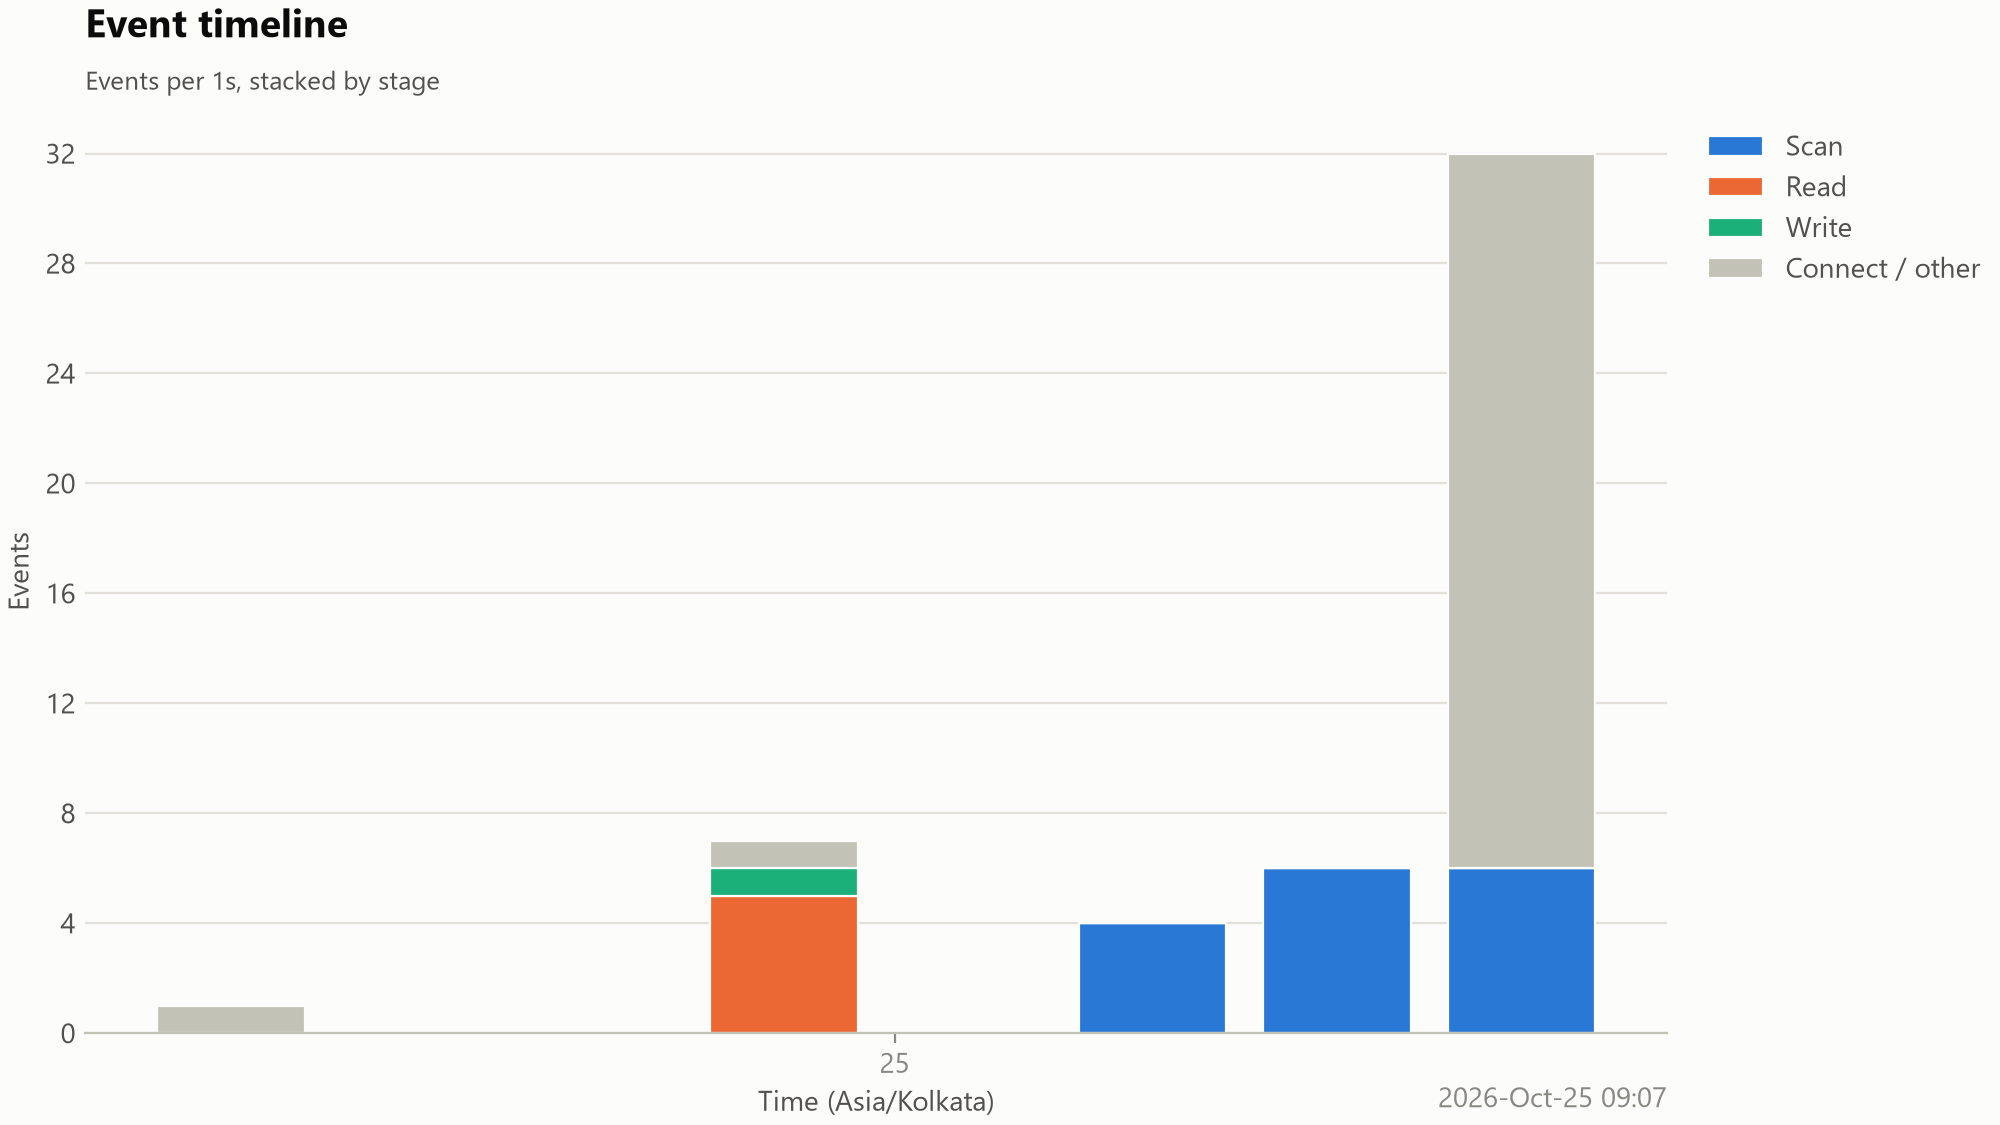
\includegraphics[width=\linewidth]{event-timeline}
    \end{column}
    \begin{column}{0.48\textwidth}
      \textbf{Parser.} \texttt{conpot.log} $\to$ a pandas table, one row per event with:
      \begin{itemize}\footnotesize
        \item protocol, request type, function code
        \item action: \textbf{scan / read / write}
        \item source IP (+ private / Docker-gateway flags)
      \end{itemize}
      \vspace{0.4em}
      147 log lines $\to$ 50 clean events, verified by a \textbf{130+ test} suite with CI.
    \end{column}
  \end{columns}
\end{frame}

\begin{frame}{Attack-sequence detection \& risk scoring}
  \begin{columns}[c]
    \begin{column}{0.5\textwidth}
      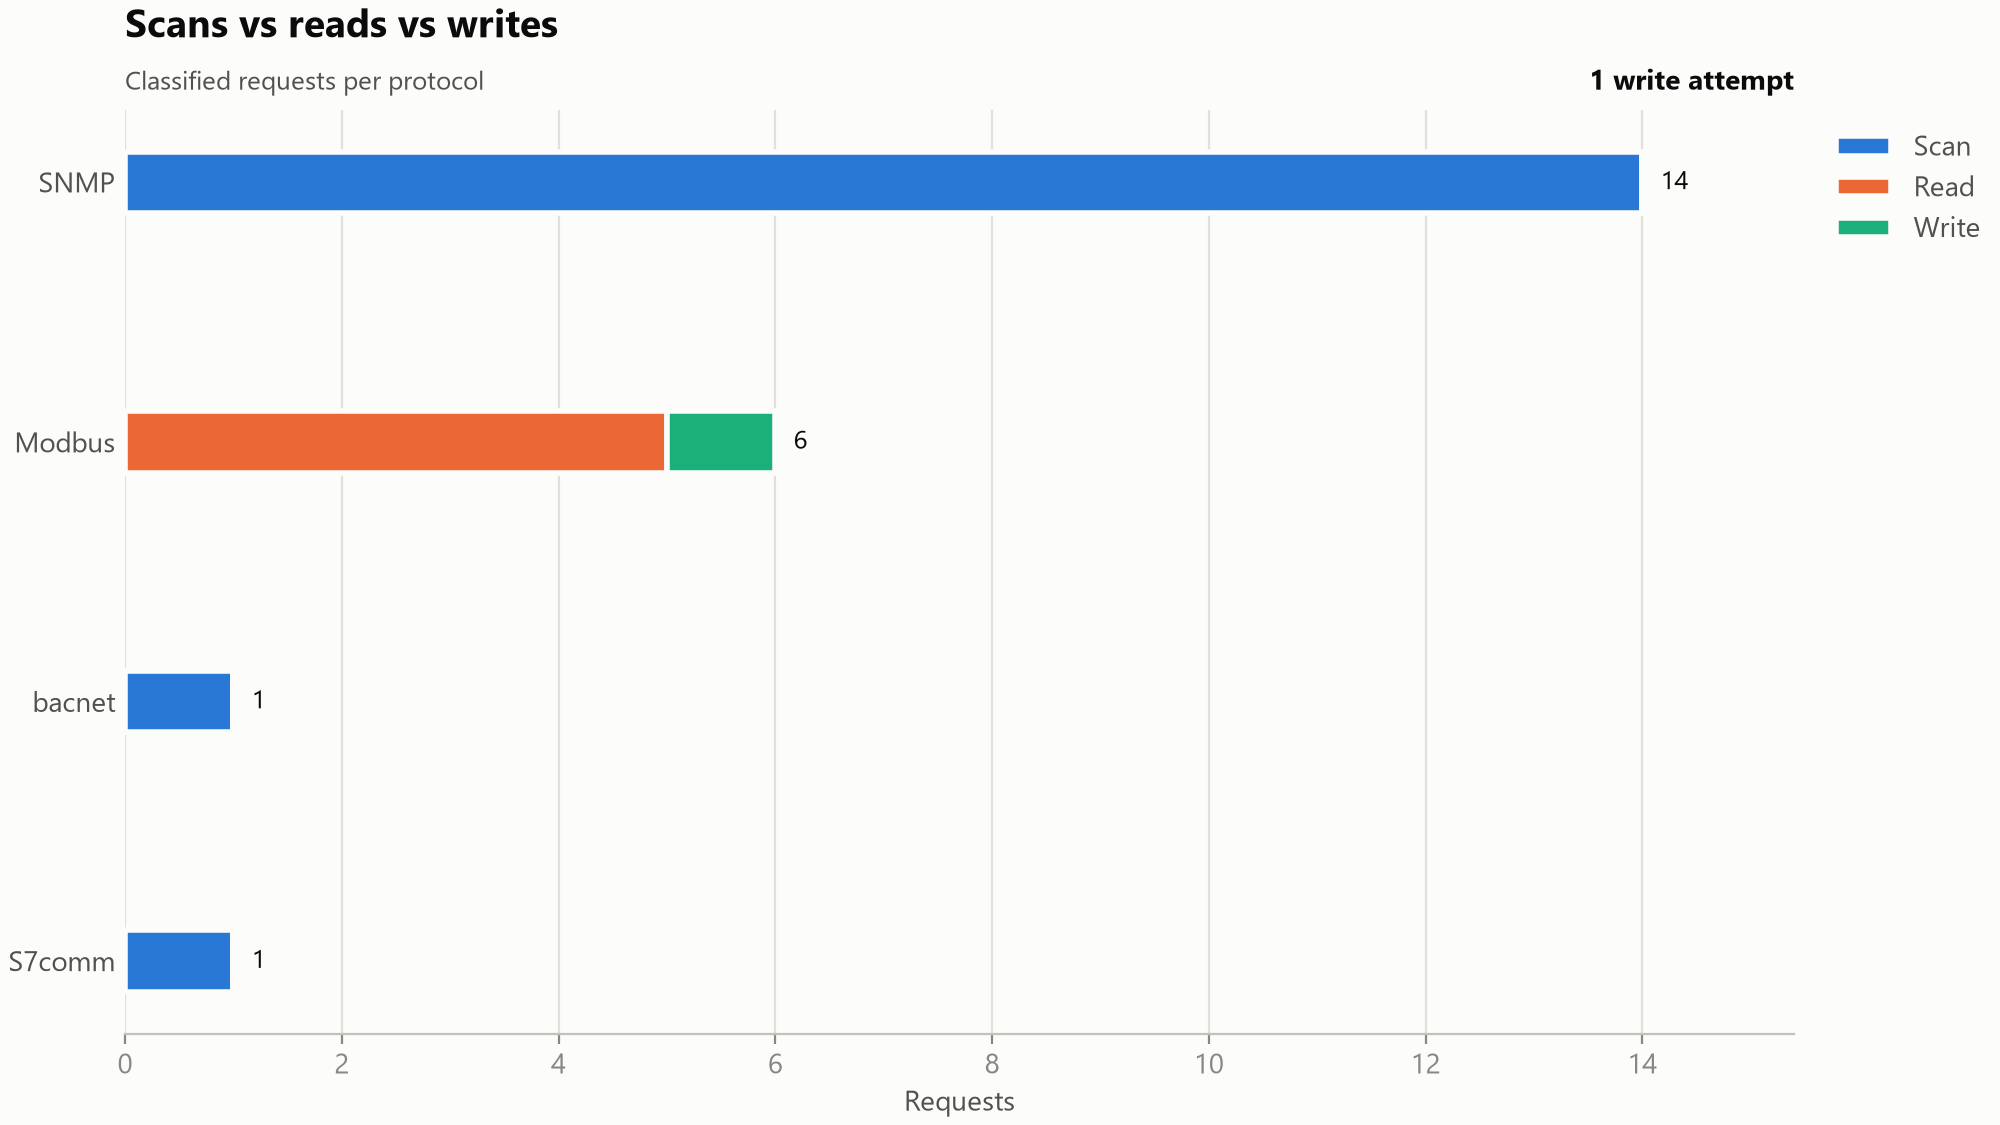
\includegraphics[width=\linewidth]{reads-vs-writes}
    \end{column}
    \begin{column}{0.5\textwidth}
      Per source IP, the detector scores risk from the attack \emph{sequence},
      multi-protocol scanning and any write attempts.
      \vfill
      \begin{block}{Our capture: \texttt{172.17.0.1}}
        Risk: \high\\
        Sequence: \textbf{\seq}\\
        Protocols: modbus, s7comm, snmp, ftp, bacnet (5)\\
        \textcolor{hpred}{Write attempt flagged}
      \end{block}
      {\footnotesize The \seq{} chain across five protocols is the classic recon-to-tamper
      pattern.}
    \end{column}
  \end{columns}
\end{frame}

\begin{frame}{Live dashboard \& attack simulator}
  \begin{columns}[T]
    \begin{column}{0.55\textwidth}
      A \textbf{Streamlit} dashboard reads the log live and shows:
      \begin{itemize}
        \item a threat-level \textbf{posture banner} + KPI tiles,
        \item interactive charts and a colour-coded risk-by-IP table,
        \item a \textbf{``Live from Docker''} source --- reads the running container directly.
      \end{itemize}
      \vspace{0.3em}
      \textbf{Attack Simulator} tab: run the attack \emph{from the UI} --- the \seq{} chain
      lights up with a PLC-status card and an attacker~$\to$~honeypot view.
      \vfill
      {\footnotesize Run with: \texttt{streamlit run dashboard/app.py}}
    \end{column}
    \begin{column}{0.45\textwidth}
      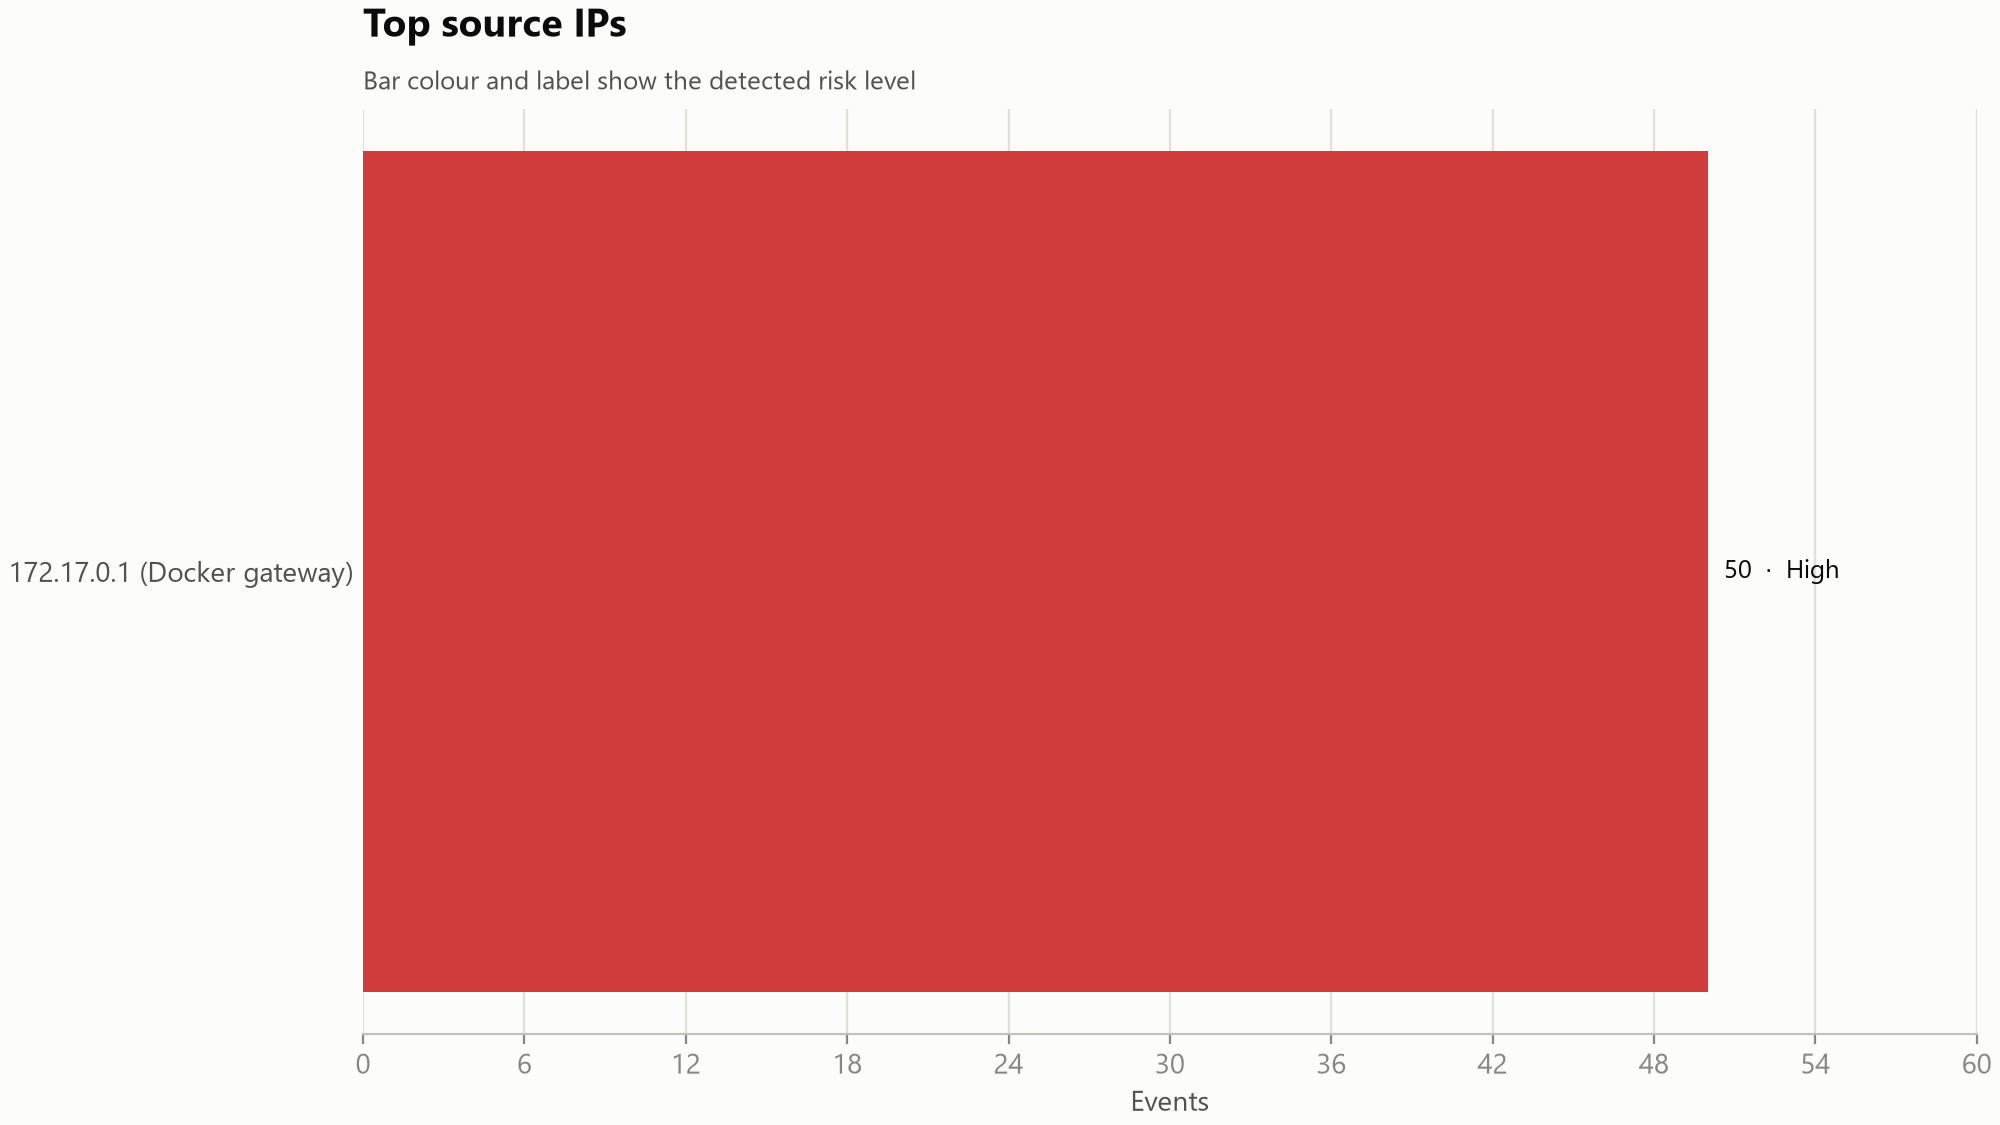
\includegraphics[width=\linewidth]{top-source-ips}
      \begin{center}{\footnotesize\textit{Top source IPs, coloured by risk}}\end{center}
    \end{column}
  \end{columns}
\end{frame}

% =====================================================================
\section{Wrap-up}
% =====================================================================
\begin{frame}{Ethics \& scope}
  \begin{itemize}
    \item Every probe targets \textbf{our own} honeypot on \textbf{localhost} --- a private,
          isolated setup; the attack console refuses any non-local target.
    \item Conpot is purpose-built to be scanned and attacked; no third party is involved.
    \item No tool here is pointed at any host we do not own or have permission to test.
  \end{itemize}
  \vfill
  \begin{block}{Why this is safe and useful}
    The honeypot has no real process to disrupt; the value is entirely in \emph{observing and
    analysing} attacker behaviour in a controlled setting.
  \end{block}
\end{frame}

\begin{frame}{Conclusion \& future work}
  \textbf{What was built}
  \begin{itemize}
    \item A Conpot ICS honeypot (Siemens S7-200) with a \textbf{custom template} that returns
          realistic Modbus data and \emph{accepts writes}.
    \item Attack traffic over \textbf{five protocols} (Modbus, SNMP, S7comm, FTP, BACnet);
          50 captured events scored \high{} risk.
    \item An automated pipeline --- parser, risk detection, interactive charts and a live
          dashboard with an \textbf{Attack Simulator} --- backed by a 130+ test suite and CI.
  \end{itemize}
  \vfill
  \textbf{Future work}
  \begin{itemize}
    \item Expose the honeypot on an isolated public-facing network to capture \emph{real}
          internet scans.
    \item Classify more protocols (TFTP, EtherNet/IP); add per-protocol attack animation and
          richer register realism.
  \end{itemize}
\end{frame}

\begin{frame}[plain]
  \vfill
  \begin{center}
    {\color{hpcyan}\rule{4cm}{1.5pt}}\\[1em]
    {\Huge\textbf{\color{ink}Thank you}}\\[0.8em]
    {\large\color{hpmuted}Questions?}\\[2em]
    {\footnotesize\color{hpmuted}Conpot ICS/SCADA honeypot --- attack \& analysis project}
  \end{center}
  \vfill
\end{frame}

\end{document}
